\section{Intro of GAN}

近年来, GAN发展迅速. 与GAN相关的论文累计数量在2016后增长迅速, 如图~\ref{fig:0101}所示. 
\begin{figure}[!htbp]
    \centering
    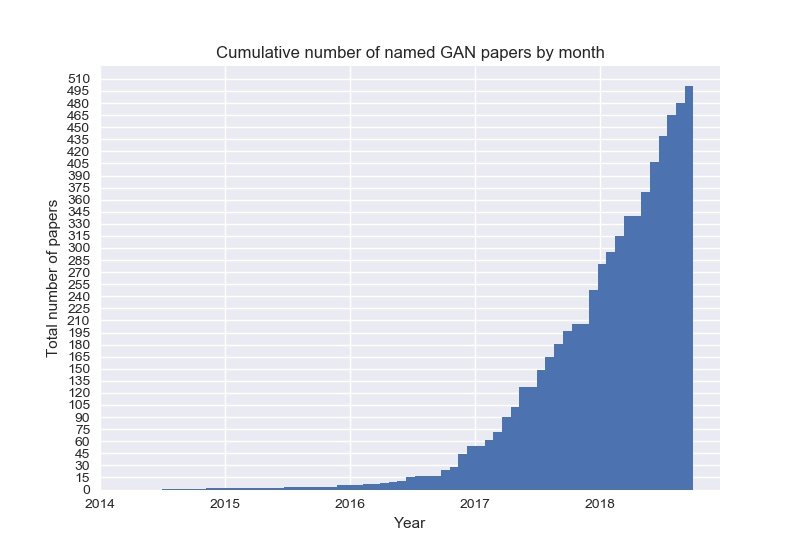
\includegraphics[height=22em]{pic/pic0101.jpg}
    \caption{GAN论文发表数量}
    \label{fig:0101}
\end{figure}

在问题~\href{https://www.quora.com/What-are-some-recent-and-potentially-upcoming-breakthroughs-in-deep-learning}{What are some recent and potentially upcoming breakthroughs in deep-learning?}中, Yann LeCun认为是GAN. 

Yann LeCunn何许人也? 卷积网络之父. 上世纪八十年代, 在博士期间, 他提出了神经网络反向传播算法的原型, 之后又开发了许多新的机器学习方法, 包括卷积神经网络, Optimal Brain Damage, regularization methods, Graph Transformer Networks 并将其应用到手写识别中, 是机器学习的大牛.

2014年, ~\href{https://github.com/goodfeli}{Ian Goodfellow}在自己蒙特利尔大学博士期间, 提出了生成对抗网络GAN. 作者本人Github头像如图~\ref{fig:0103}. 

\begin{figure}[!htbp]
    \centering
    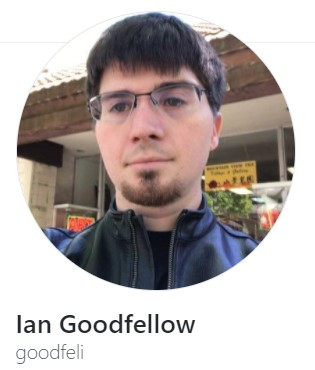
\includegraphics[height=12em]{pic/cover.jpg}
    \caption{Ian Goodfellow}
    \label{fig:0103}
\end{figure}


% \begin{figure}[!htbp]
%     \centering
%     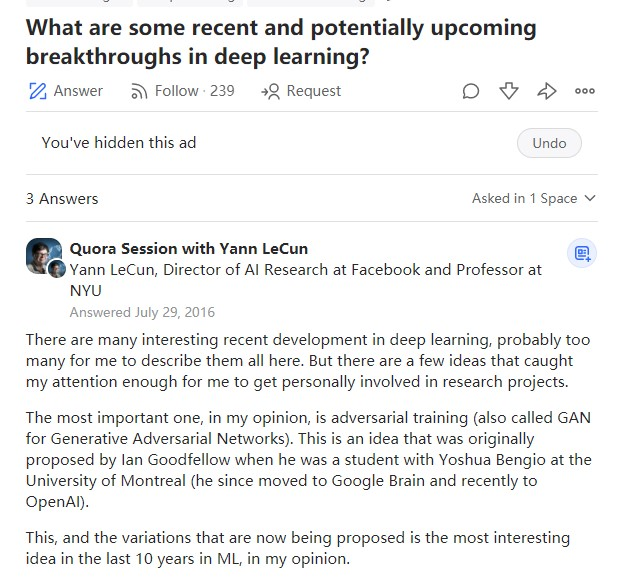
\includegraphics[height=22em]{pic/pic0102.jpg}
%     \caption{Quora 问答}
%     \label{fig:0102}
% \end{figure}

